\subsection{Schwerpunktverteilung mit Gleitkommazahlen}
\begin{table}[h!]
    \hspace{-0.5cm}
    \begin{tabular}{ | l | c | c | c | c |}
        \hline
        Konfiguration & Beste & Unter 60 kB & Unter 28 kB & Unter 14 kB \\\hline
        Ensemble-Methode & Boosting & Boosting & RandomForest & Bagging  \\\hline
        Maximalhöhe & 20 & 19 & 10 & 7 \\\hline
        Waldgröße & 10 & 6 & 4 & 3 \\\hline
        min\_samples\_leaf & 8 & 8 & 2 & 8 \\\hline
        Programmgröße in Bytes & 83304 & 43678 & 20188 & 6656 \\\hline
        Genauigkeit Testmenge von Klisch & 94,8\% & 94.8\% & 89,6\% & 87,5\% \\\hline
        Genauigkeit Gestentestmenge & 97,0\% & 96,1\% & 95,6\% & 94,1\% \\\hline
        Genauigkeit Nullgestentestmenge & 92,2\% & 91,1\% & 88,8\% & 89,9\% \\\hline
    \end{tabular}
    \caption{Beste Konfigurationen der Schwerpunktverteilung mit Gleitkommazahlen.}
    \label{tab:schwerpunktverteilung_float}
\end{table}
\begin{figure}[h!]
    \centering
    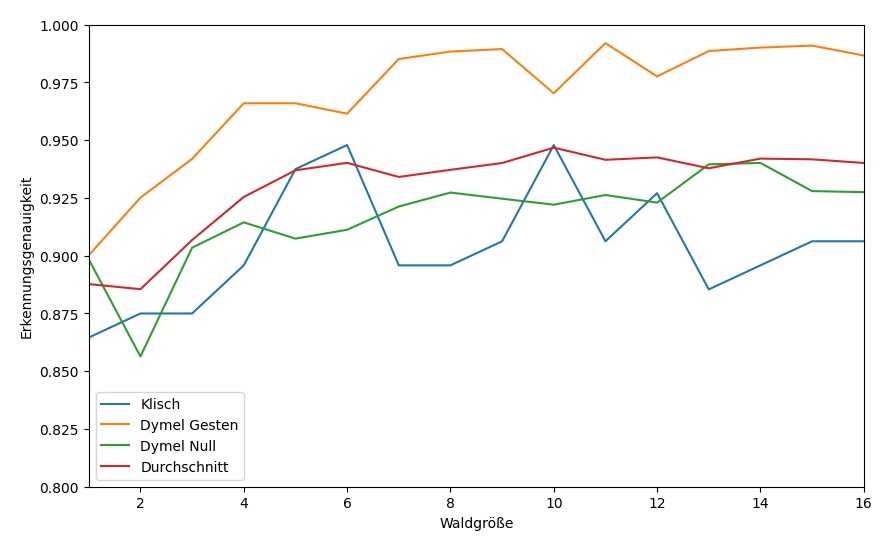
\includegraphics[width=\linewidth]{images/cocd_float_acc_per_size.png}
    \caption{Die beste summierte Erkennungsgenauigkeit pro Waldgröße der Schwerpunktverteilung mit Gleitkommazahlen.}
    \label{fig:cocd_float_per_forest_size}
\end{figure}
Die Featuremenge Schwerpunktverteilung mit Gleitkommazahlen folgt der Definition aus Sektion \ref{sec:schwerpunktverteilung} und beinhaltet insgesamt 10 Einträge, wobei jeweils 2 Einträge die X und Y
Koordinate des Schwerpunktes darstellen in insgesamt 5 Zeitfenstern.
\newline
\newline
Die beste Konfiguration wurde mit der Boosting Ensemble-Methode erzielt (siehe Tabelle \ref{tab:schwerpunktverteilung_float}). Mit einer Erkennungsgenauigkeit von $94,8\%$ auf der Testmenge von Klisch
ist dieser Ansatz nur $5,2\%$ schlechter als das neuronale Netz von Giese \cite{gieseThesis}. Es ist anzumerken, dass mit einer kleineren Trainingsmenge ohne Nullgesten eine Lösung gefunden wurde, die
$97,9\%$ erzielte und damit nur $2,1\%$ schlechter ist. Außerdem werden $92,2\%$ der Nullgestentestmenge von Dymel korrekt klassifiziert und $97\%$ der Gestentestmenge von Dymel. Die anderen
Ensemble-Methoden sind nur marginal schlechter.
\newline
\newline
Alle Konfigurationen sind ohne Optimierung aber zu groß um kompeliert zu werden. Aus diesem Grund wurden die gleichen Konfigurationen mit Festkommazahlen und dem diskreten Wahlklassifizierer reevaluiert.
TODO: Evaluieren, evtl. kleinere Waldgröße nutzen, e.g. 6 und mit Graphen begründen.
\newline
\newline
In Abbildung \ref{fig:cocd_float_per_forest_size} kann man einen Anstieg der Erkennungsgenauigkeit mit zunehmender Waldgröße auf den Testmengen von Dymel erkennen. Bis zu einer Waldgröße von 6 gilt das
auch für die Testmenge von Klisch, allerdings fängt sie ab dort an zu schwanken.

\iffalse
!! Merke beste Klisch Genauigkeit an. Problem beim finden mit größerer Trainingsmenge

Pro Analyse:
* Explain the featureset a little
* Beste Konfiguration specs, pro Ensemble-Methode
=> Acc und size vor und nach optimierung
* Verschiedene Waldgrößen verglichen
\fi